\documentclass[11pt,a4paper,twocolumn]{article}
\usepackage{paperstyle}
% Generated by scripts/analyze_results.py; do not edit.
\newcommand{\BaselineRate}{22.5}
\newcommand{\CbeRate}{23.6}
\newcommand{\TaskDelta}{+1.12}
\newcommand{\CILower}{-2.6}
\newcommand{\CIUpper}{+4.9}
\newcommand{\OutputReduction}{5.6}
\newcommand{\InputIncrease}{18.3}
\newcommand{\WorkIncrease}{68}
\newcommand{\MedianPreparation}{70}
\newcommand{\MixedEither}{25}
\newcommand{\BaselineMixed}{18}
\newcommand{\CbeMixed}{19}
\newcommand{\CompleteTasks}{89}
\newcommand{\BaselineCompletedCalls}{17,065}
\newcommand{\CbeCompletedCalls}{14,750}

% Generated; no new trials.
\newcommand{\BaselinePublic}{240}
\newcommand{\CbePublic}{234}
\newcommand{\BaselinePublicRate}{91.6}
\newcommand{\CbePublicRate}{90.0}
\newcommand{\BaselinePublicOnly}{180}
\newcommand{\CbePublicOnly}{174}
\newcommand{\HiddenPrivateDifferences}{30}

\hypersetup{pdftitle={Computation and Boundary Evidence for Scientific Software Repair},pdfauthor={Rajarshi Ghoshal}}
\title{Computation and Boundary Evidence for Scientific Software Repair}
\author{Rajarshi Ghoshal\\\texttt{rajarshi.ghoshal1@gmail.com}\\PhD applicant research task --- Graz University of Technology}
\date{}
\setlength{\parindent}{0pt}
\setlength{\parskip}{2pt}
\captionsetup{hypcap=false}
\newcommand{\smalltable}{\fontsize{8.7}{10.7}\selectfont\setlength{\tabcolsep}{3pt}\renewcommand{\arraystretch}{1.12}}
\begin{document}
\raggedbottom
\maketitle

\begin{abstract}
Scientific software repair requires identifying relevant computations while preserving expected behaviour. We ask whether making repository-derived computational evidence directly queryable improves repair under a matched agent budget. Computation and boundary evidence (CBE) combines public-reproducer tracing with static extraction of expressions, conditions, documented definitions, and library-call boundaries, without preprocessing model calls. On 89 SWE-bench Science tasks with three runs per arm, baseline and CBE solve 60/267 and 63/267 attempts; the paired confidence interval spans zero. CBE records \OutputReduction\% less output generation but greater input consumption and work time. Discipline-level summaries locate opposing changes, and contrasting patches illustrate incomplete calculation repair and interface-preservation failures. This proof of concept exposes a design limitation: locating computational evidence does not establish that it covers the task's correctness requirements. We discuss this limitation through the benchmark's task paradigms, without claiming unmeasured paradigm-specific effects.
\end{abstract}

\section{Introduction}

Task 103 in SWE-bench Science asks an agent to repair a composite-laminate stiffness calculation in pyNastran. In the reported attempts, expanding the ply iteration without correcting the accumulation formula passes the public reproducer but fails the complete private suite. The example motivates making the computation surrounding a candidate repair directly inspectable, rather than leaving the agent to reconstruct it through text search.

CBE organizes this repository-derived evidence before repair and exposes it through three query endpoints beside the usual shell tools. Public execution observations guide source selection; static extraction links computations, conditions, definitions, and call boundaries. The baseline uses the same model, budget, and containers without this evidence store.

Our research question is whether this additional representation improves complete repair. The contributions are the preparation pipeline, query interface, and replicated comparison. We analyze both successful and unsuccessful changes to understand the representation's scope, not to assume that every scientific task requires the same evidence.

CBE draws on traceability~\citep{niu2023ablots,niu2023rat,niu2025tvr,pan2025coverage}, code property graphs~\citep{yamaguchi2014cpg}, scientific model extraction~\citep{pyarelal2020automates,skema2024gromet}, and incremental parsing~\citep{treesitter2024}. We evaluate on SWE-bench Science~\citep{xu2026science} with DeepSeek V4.1 Flash~\citep{deepseek2026}; SWE-bench~\citep{jimenez2024swebench,yang2024swebenchverified} and SciCode~\citep{tian2024scicode} are related benchmarks.

\section{What CBE provides}
\label{sec:method}

The pipeline has three stages (Figure~\ref{fig:method}): trace, extract, query.

\paragraph{Trace.}
Run the public \texttt{reproduce.py} under an observer. The observer records which functions execute, guiding file selection for extraction. No model calls. Median duration: \MedianPreparation{}\,s of the 1800\,s budget.

\paragraph{Extract.}
Tree-sitter~\citep{treesitter2024} parses Python ASTs for scopes, assignments, binary expressions, return anchors, and branches. Joern handles C, C++, Fortran, and Cython where available; explicit fallback otherwise. External calls are labelled with their provider as interface assumptions, not correctness guarantees. Unresolved callees stay \texttt{unknown\_external}.

Table~\ref{tab:representation} shows what CBE extracts for task 103 (pyNastran) --- the opening example. The computation record links the accumulation at line 1003 to its return anchor. The boundary record identifies the numpy call and its scope.

\begin{minipage}{\columnwidth}
\captionof{table}{CBE evidence records for task 103 (pyNastran).}
\label{tab:representation}
\smalltable
\begin{tabularx}{\columnwidth}{@{}p{1.65cm}X@{}}
\toprule
Record & Content \\
\midrule
Computation & Scope, expressions, result anchors: accumulation at line 1003 $\to$ \texttt{return ABD} at 1015. \\
Condition & \texttt{len(z0) == len(z1)} at line 987. \\
Definition & Documented public behavior (not execution trace). \\
Boundary & \texttt{np.radians(thetad)} at line 979: provider \texttt{numpy}, caller-side scope. \\
\midrule
\multicolumn{2}{@{}l}{\textbf{Query interface (alongside ordinary shell)}} \\
\texttt{find} & Keyword search over symbols, docstrings, and expressions. \\
\texttt{inspect} & Structured view: dependencies, conditions, boundaries. \\
\texttt{note} & Scratchpad for working hypotheses; never gates repair. \\
\bottomrule
\end{tabularx}
\end{minipage}

\paragraph{Query and repair.}
The agent accesses the three endpoints alongside its normal shell utilities. \texttt{find} searches the indexed structure; \texttt{inspect} retrieves computation scopes and boundary details; \texttt{note} records a working hypothesis without blocking repair. Inspection refreshes after each edit; the preparation trace stays fixed.

\section{Protocol}
\label{sec:protocol}

SWE-bench Science contains 119 tasks across 20 disciplines~\citep{xu2026science}. We use 30 tasks for development and evaluate the remaining 89, spanning 18 disciplines. Each task runs three times per arm (534 verified attempts). Both arms share the conditions in Table~\ref{tab:setup}.

\begin{minipage}{\columnwidth}
\captionof{table}{Shared evaluation parameters.}
\label{tab:setup}
\smalltable
\begin{tabularx}{\columnwidth}{@{}p{1.65cm}X@{}}
\toprule
Component & Detail \\
\midrule
Model & DeepSeek V4.1 Flash~\citep{deepseek2026}; temperature 0; \texttt{PYTHONHASHSEED=0}. \\
Replicates & 89 tasks $\times$ 3 runs = 267 per arm; 534 verified. \\
Budget & 1800\,s, including preparation. \\
Verification & Separate container, 1800\,s. Private tests not visible. \\
Network & None. \\
Baseline & Shell tools + public task material. \\
CBE & Same + evidence store + three query endpoints. \\
\bottomrule
\end{tabularx}
\end{minipage}

A solve is a successful official verifier reward, not merely a passing public reproducer or private-test subset. All reported attempts have verdicts. We bootstrap per-task rate differences with 20,000 resamples and a fixed analysis seed; the paired sign test excludes ties.

\section{Results}
\label{sec:results}

\paragraph{Aggregate comparison.}
Baseline solves 60 of 267 verified attempts; CBE solves 63 of 267 (Table~\ref{tab:main}). The paired interval spans zero: the observed difference does not establish an aggregate benefit or equivalence.

\begin{minipage}{\columnwidth}
\captionof{table}{Baseline solves 60, CBE solves 63. CBE generates \OutputReduction\% fewer output tokens.}
\label{tab:main}
\smalltable
\begin{tabular*}{\columnwidth}{@{\extracolsep{\fill}}lrr@{}}
\toprule
Metric & Baseline & CBE \\
\midrule
% Generated from verified receipts (run.json stage summaries, not per-call records).
Scheduled attempts & 267 & 267 \\
Exact repairs / verdicts & 60/262 & 60/260 \\
Exact-repair rate & 22.9\% & 23.1\% \\
Private tests passed & 2315/3167 & 2226/3148 \\
Output tokens (M) & 12.01 & 10.36 \\
Input tokens (M) & 838.0 & 878.3 \\
Mean work per attempt (s) & 1236.6 & 1306.9 \\
\bottomrule

\end{tabular*}
\vspace{3pt}
{\fontsize{8.2}{9.8}\selectfont
Paired task-rate diff: \TaskDelta{}\,pp; 95\% bootstrap $[\CILower,\CIUpper]$\,pp; sign $p=1.00$. All 534 attempts verified (267 per arm); mean work averages runtime across attempts with usage records.}
\end{minipage}

\paragraph{Resource shift.}
74 tasks tie, 8 favour CBE, 7 favour baseline. Output drops \OutputReduction\% (12.81M vs.\ 13.56M tokens); input rises \InputIncrease\%; work takes \WorkIncrease\,s longer. These recorded resource changes describe a trade-off, not an overall efficiency improvement or a measurement of search behaviour.

\paragraph{Hidden partial changes.}
Even among exact ties, behaviour differs: \HiddenPrivateDifferences{} of 74 differ in private-test pass fractions (Table~\ref{tab:partial}). CBE passes more tests on nine tasks; baseline passes more on 20.

\begin{minipage}{\columnwidth}
\captionof{table}{Task counts by the direction of exact-repair and private-test pass-fraction differences.}
\label{tab:partial}
\smalltable
\begin{tabular*}{\columnwidth}{@{\extracolsep{\fill}}lrrr@{}}
\toprule
& \multicolumn{3}{c}{Private-test pass fractions} \\
Exact rate & Baseline higher & Equal & CBE higher \\
\midrule
% Generated from per-task exact and mean private rates.
Baseline higher & 7 & 0 & 1 \\
Equal & 21 & 44 & 9 \\
CBE higher & 0 & 0 & 7 \\
\bottomrule

\end{tabular*}
\end{minipage}

\clearpage
\twocolumn[{\begin{minipage}{\textwidth}
\section{Task-level variation and evidence scope}
\label{sec:domains}
\centering
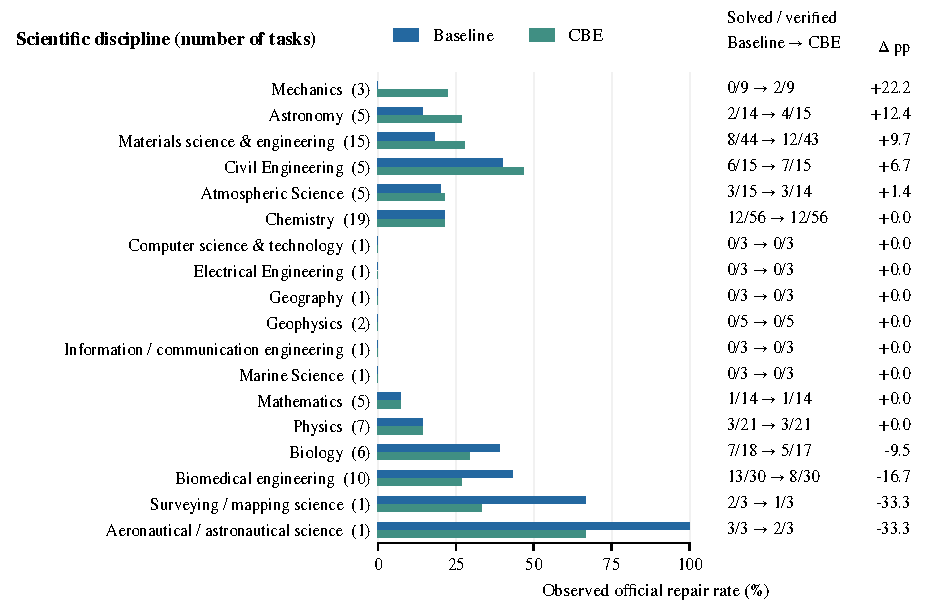
\includegraphics[width=\textwidth]{figures/domain_outcomes.pdf}
\captionof{figure}{Solve-rate difference (CBE $-$ Baseline) for the ten disciplines with non-zero change. Task counts in parentheses. Eight disciplines with identical solve rates across arms are omitted.}
\label{fig:domains}
\end{minipage}\vspace{9pt}}]

Figure~\ref{fig:domains} shows gains in six disciplines and losses in four. Mechanics' gain comes entirely from task 103, while the materials-science gain spans DeePTB, deepmd-kit, and dpdata. Biology's net loss comes from biopython in the current comparison. Each of the two largest negative differences represents one task. These descriptive groups locate the observed changes; discipline alone does not explain why a repair succeeds or fails.

\paragraph{Task demands and representation scope.}
The benchmark distinguishes \emph{Issue-driven}, \emph{Expert-exploratory}, and \emph{Engineering-integration} tasks~\citep{xu2026science}. These describe how a problem is posed, not its scientific discipline or the obligations of its eventual patch. A known defect still requires regression preservation; investigating an anomaly requires comparing possible explanations; integration requires checking behaviour across modules. Computation and call records may support all three, but do not by themselves establish that the relevant evidence is complete. We use these paradigms to discuss scope; our analysis does not include per-task paradigm annotations, so we report no subgroup rates.

\paragraph{Replication.}
Baseline and CBE never solve 60 and 59 tasks, respectively. Outcomes are mixed on 18 baseline and 19 CBE tasks; 11 tasks succeed in all three runs for each arm. The repeated outcomes make within-task variation visible without defining a fixed resolution threshold.

\paragraph{Task-localized, not task-adaptive.}
The reproducer guides CBE toward code exercised by the task, but the evidence schema does not explicitly adapt to these different demands. The repair agent must still determine whether the extracted records explain the discrepancy and cover the behaviours a change must preserve. The following cases examine this gap between access to relevant code and a complete repair.

\vspace{4pt}
\begin{minipage}{\columnwidth}
\centering
\begin{tikzpicture}[x=1mm,y=1mm,
  every node/.style={font=\fontsize{7.5}{9}\selectfont},
  box/.style={draw=baselineblue!60,fill=baselineblue!4,rounded corners=.8mm,align=center,minimum height=7mm,inner sep=1.5mm},
  arr/.style={-{Stealth[length=1.2mm]},draw=baselineblue!70,line width=.5pt}]
\node[box,text width=20mm] (a) at (0,0) {\textbf{Trace}\\reproducer};
\node[box,text width=20mm] (b) at (28,0) {\textbf{Extract}\\AST + CPG};
\node[box,text width=20mm] (c) at (56,0) {\textbf{Store}\\evidence};
\node[box,text width=20mm,draw=cbeteal!60,fill=cbeteal!4] (d) at (56,-12) {\textbf{Query}\\find / inspect / note};
\node[box,text width=20mm] (e) at (28,-12) {\textbf{Repair}\\edit + test};
\draw[arr] (a)--(b); \draw[arr] (b)--(c); \draw[arr] (c)--(d); \draw[arr] (d)--(e);
\end{tikzpicture}
\captionof{figure}{CBE pipeline: trace the reproducer, extract computation structure, store it, then the agent queries and repairs.}
\label{fig:method}
\end{minipage}

\clearpage
\twocolumn[{\begin{minipage}{\textwidth}
\section{Case studies}
\label{sec:cases}
\centering
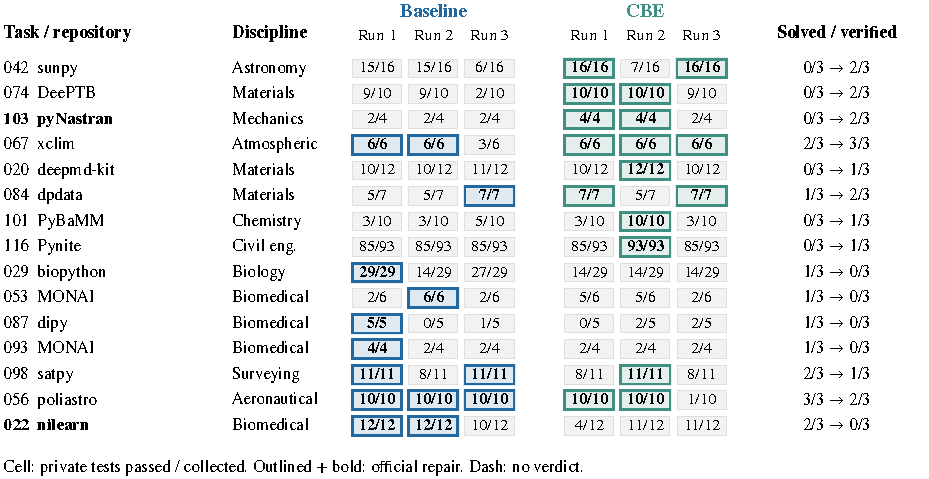
\includegraphics[width=\textwidth]{figures/trial_test_matrix.pdf}
\captionof{figure}{Per-run private-test pass fractions for every task whose solve rate differs between arms. Outlined bold cells are official solves; bold task labels are the two cases below.}
\label{fig:trials}
\vspace{3pt}
\captionof{table}{Comparison of generated patches for divergent case studies.}
\label{tab:cases}
{\fontsize{8}{9.5}\selectfont\setlength{\tabcolsep}{2.5pt}\renewcommand{\arraystretch}{1.05}
\begin{tabularx}{\textwidth}{@{}p{1.1cm}XXX@{}}
\toprule
Task & Baseline & CBE & Insight \\
\midrule
103 pyNas\-tran & Expand ply iteration; keep original B/D accumulation. All pass public. & Two fix both expansion and B/D; third keeps old accumulation. & The public check does not distinguish partial from complete repairs of this calculation. \\
\addlinespace[1pt]
022 nilearn & Successful patches add label aggregation while preserving the nearest-neighbour path. & Two alter argument handling (11/12 private); the third passes 4/12. & Reaching relevant aggregation code is not sufficient to preserve existing interface behaviour. \\
\bottomrule
\end{tabularx}}
\end{minipage}\vspace{2pt}}]

\paragraph{Task 103 (pyNastran).}
Figure~\ref{fig:trials} separates incomplete fixes from complete repairs. All baseline attempts pass the public check but only two of four private tests. The two successful CBE patches change both expansion and accumulation. This contrast supports examining repair completeness, rather than treating localization as the only obstacle.

\paragraph{Task 022 (nilearn).}
The successful baseline patches preserve the existing nearest-neighbour path while adding label aggregation. Two CBE patches also alter argument handling and pass 11/12 private tests; the third passes 4/12. These post-hoc patch comparisons suggest a compatibility concern, but do not establish that reading computational evidence caused it.

\section{Limitations and conclusion}
\label{sec:conclusion}
The principal limitation is the extractor's scope. CBE prepares a task-localized view of repository evidence, but does not explicitly determine which kinds of evidence the repair requires or whether the extracted view is sufficient. Documented definitions and predicates provide semantic cues, not a complete specification of scientific meaning or compatibility requirements. The agent must still form and test hypotheses and check the implications of edits across the relevant workflow.

The public trace covers observed execution, while extraction fallbacks and unresolved calls limit structural coverage. A named external provider is an interface assumption, not verification. Nor does observing three successful attempts demonstrate generalization beyond the verifier. No component ablation isolates tracing, extraction, or querying. Most evaluated tasks are Python, and the comparison uses one model and scaffold.

CBE yields similar observed repair rates with a resource trade-off. The cases motivate investigating whether the evidence supplied covers the repair obligation; they do not establish universal benefits for calculation tasks or harms for interface tasks. Extending evidence relevance and completeness is a design direction, not a result of this evaluation.

\section{AI Assistance}
ChatGPT and Oh My Pi assisted with coding, debugging, analysis, and plotting. Code, receipts, and per-task outcomes: \url{https://github.com/rajarshighoshal/computation-boundary-evidence}.

\clearpage
\bibliography{references}
\end{document}
